\begin{FlushLeft}
    \section{Program Testing}
    \subsection{Testing Tables}
    \subsubsection{Targeted Testing Areas}

    \normalsize
    In order to ensure that my NEA conforms to my objectives this following section will test each of them one at a time. As well as this I will test to make sure that each part of the final solution works together and produces the desired and expected output. \\
    An overview of the sections I will test are:
    \begin{enumerate}
        \item User Map Inputs and Subsequent Outputs
        \begin{enumerate}
            \item Loading In Image Files
            \item Creating The Save File
            \item Options Given To User
            \item Conversion To Graph
            \item Error Handling 
        \end{enumerate}\bk
        \item Canny Edge Detection Operations
        \begin{enumerate}
            \item User Variables
            \item Constructor Arguments
            \item Full Flow Thorough
            \item Individual Method Calls
            \item Exceptions
        \end{enumerate}\bk
        \item Road Detection
        \begin{enumerate}
            \item User Variables
            \item Constructor Arguments
            \item Full Flow Through
            \item Individual Method Calls
            \item Exceptions
        \end{enumerate}\bk
        \item Graph Traversal
        \begin{enumerate}
            \item Different Node Placements
            \item Different Algorithms
            \item Other Graph Settings
        \end{enumerate}\bk
        \item Logging and Saves
        \begin{enumerate}
            \item Validity Of Save Files
            \item Contents of Log Files
            \item Save Settings
        \end{enumerate}\bk
        \item Miscellaneous Items + GUI
        \begin{enumerate}
            \item GUI Elements
            \item Matrix Functions
            \item Extensions and Utilities 
            \item Structures
        \end{enumerate}
    \end{enumerate}
    \bk

    It should be noted that in the following tests do not explicitly test objective 5 however it can be seen through out the video that this objective has been met. From the icon being clear to the user interface clearing. I believe this combined and the constant evidence shown through the video allows me to come to the conclusion that objective 5 has been met.
    

    \bk
    \setlength\LTpre{0pt}

    \subsubsection{User Inputs and Outputs Testing Table}
    \bk
    \normalsize
    \begin{longtable}{| C{0.6cm} | C{2.5cm} | C{4.75cm} | C{4.75cm} | L{1cm} | L{1.4cm} |}
    \hline
    {\footnotesize Test No.}  & Name & Input Data / Description & Expected Output & Pass Fail & Test Evidence \\
    \hline\hline
    \multicolumn{6}{| l |}{\textbf{1.1.(2)} The program should be able to parse a map from a file including...} \\
    \hline
    \rn  & Entering a JPG & Enter the test image as a JPG into the "New Image" promp. & The program should accept the image and be able to process it and show it to the user in the "Preview Form" & Pass & TODO \\
    \hline
    \rn  & Entering a PNG & Enter the test image as a PNG into the "New Image" promp. & The program should accept the image and be able to process it and show it to the user in the "Preview Form" & Pass & TODO \\
    \hline
    \rn  & Entering a BMP & Enter the test image as a BMP into the "New Image" promp. & The program should accept the image and be able to process it and show it to the user in the "Preview Form" & Pass & TODO \\
    \hline
    \rn  & Entering a TIFF & Enter the test image as a TIFF into the "New Image" promp & The program should accept the image and be able to process it and show it to the user in the "Preview Form" & Pass & TODO \\
    \hline  
    \multicolumn{6}{| l |}{\textbf{1.1.1} A photograph of an map} \\
    \hline
    \rn  & Entering a Photograph & Enter a photograph into the "new image prompt" & The program should accept the image and be able to process it and show it to the user in the "Preview Form" & Pass & TODO \\
    \hline    
    \multicolumn{6}{| l |}{\textbf{1.1.3} A hand drawing of suitable quality (if it is not a message should be shown)} \\
    \hline
    \rn  & Entering a Hand Drawing & Enter a hand drawing into the "new image prompt" & The program should accept the image and be able to process it and show it to the user in the "Preview Form" & Pass & TODO \\
    \hline    
    \multicolumn{6}{| l |}{\textbf{1.4} A hand drawing of suitable quality (if it is not a message should be shown)} \\
    \hline
    \rn  & Entering a Small Image (less than 200x200) & Resize test image to be less than 200x200 and then input that into the "New Image" prompt & The program should reject the image and instruct the user as to how to fix the issue. & Pass & TODO \\
    \hline
    \rn  & Entering an Invalid Image Path & At the "New Image" prompt an invalid file path should be entered. This test should be repeated with different invalid paths to make sure that all cases are accounted for. & The program should reject all of these inputs without crashing. & Pass & TODO \\
    \hline  
    \rn  & Entering an Local Path & The test described described here would consist of a path in the form "../../image.png" for example. & The program should be able to process this path and show the image to the user in the "Preview Image" form. & Pass & TODO \\
    \hline
    \rn  & Entering a Valid Save Path & A valid save file path should be entered, use the test image save "save.vmap". & the program should accept this input and show the "Recalled Image" options. & Pass & TODO \\
    \hline
    \rn  & Entering an Invalid Save Path & An invalid save file path should be entered. This can be any path ending with "/<something>.vmap" & The program should error and instruct the user how to fix the issue. & Pass & TODO \\   
    \hline
    \rn  & Try to Escape Bounds of Option Selector & When in the main menu attempt to go out of bounds of the menu and then select a non existent element. & The option function should not allow the user to go out of the options presented. & Pass & TODO \\
    \hline
    \rn  & Try to Break inputs through pre-clicking enter. & When going through menus repeatably click the enter key in order to attempt to get the program to error. This can include clicking misc keys as well as enter. & The program should handle all of these inputs before it then waits for non spammed inputs. It should not error. & Pass & TODO \\
    \hline
    \rn  & Remove Characters from Input & When a text input is required, for example the new image prompt when a path is entered, there is a chance that the user could have entered a mistake. Enter random characters then click "Backspace" to remove characters. & The characters should be removed and no error should occur if the backspace is clicked when the carat is at the end it should not error, & Pass & TODO \\
    \hline
    
    \multicolumn{6}{| l |}{\textbf{1.3} The inputted map should be converted into a graphs} \\
    \hline
    \rn  & Graph Constructor & Inside the testing menu run the test "Manual Graph", this should generate a predefined graph which contains the nodes and connections as follows. & \begin{enumerate}[label=\Alph*:]
        \item D
        \item F, C
        \item B
        \item A, E, G
        \item D, H
        \item B, G
        \item D, F
        \item E
    \end{enumerate} & Pass & TODO \\
    \hline

    \rn  & ToGraph Method & On a small test image the function extension .ToGraph should be run. & The outputted graph should contain the following nodes, {(0,2), (1,2), (2,0), (2,1), (2,2), (2,3), (2,4), (2,5), (3,2), (4,2), (5,2)} & Pass & TODO \\
    \hline
    
    \end{longtable}
    \BK


    \setcounter{magicrownumbers}{0}
    \subsubsection{Canny Edge Detection Testing Table}
    \bk
    \normalsize
    \begin{longtable}{| C{0.6cm} | C{2.5cm} | C{4.75cm} | C{4.75cm} | L{1cm} | L{1.4cm} |}
    \hline
    {\footnotesize Test No.}  & Name & Input Data / Description & Expected Output & Pass Fail & Test Evidence \\
    \hline\hline 
    \multicolumn{6}{| l |}{\textbf{2.1} At each stage of the edge detection an image should be produced} \\
    \hline
    \rn  & Canny Edge Detect Save Images & Run through a full map detection and at the prompt when it asks if the user would like to save an image at each stage of the canny edge detection select yes then run the canny edge detection. & Each stage of the edge detection will have an image saved in the runs/<id> folder. & Pass & TODO \\
    \hline
    \multicolumn{6}{| l |}{\textbf{2.3.1} AThere should be presets to allow quicker processing} \\
    \hline
    \rn & Run A Preset & The test image should be input at the "New Image" prompt. When it comes to picking how the edges should be picked the preset "Screenshot" should be selected. & The program should perform Canny Edge Detection without prompting the user for variables. It should return to user control at the "Invert Image" stage. & Pass & TODO \\
    \hline
    \multicolumn{6}{| l |}{\textbf{2.3} The edge detection must have the option to be multi threaded.} \\
    \hline
    \rn  & Cancel A Run & As above the test image should be entered. Both when it comes to the edge picking "Multi-threaded" then entering values then when the program confirms to continue select "No", and when the image is first read selecting "No" when the "Correct Image" prompt shows. & The program should stop running the current image and error with the reason "You asked for the processing of your map to stop." Then it should return to the main menu. & Pass & TODO \\
    \hline
    \multicolumn{6}{| l |}{\textbf{2.2} Between each stage the user should be able to repeat the last step in order to change parameters.} \\
    \hline
    \rn  & Enter Invalid Values & During the selection of canny edge detection variations "Multi-threaded" should be chosen. When the program prompts for user inputs a variety of invalid ones should be provided. For example "test", "999999", "1s", "newline", "zero" etc... & The program should check to see if these inputs are within the bounds of the required variables and if they are not it will assume a default value and inform the user. & Pass & TODO \\
    \hline
    \rn  & Enter Valid Values & Same prompt as above, in the multi-threaded canny edge detection variables. However this time valid values should be input, these should test the bounds of the inputs as prompted by the program. & The program should accept these changed values and notify the user of what they have changed too. & Pass & TODO \\
    \hline
    \end{longtable}

    
    \textit{The following tests ending in "method" are run one at a time during the slow, single threaded version of canny edge detection with the exception of the Gradient calculation with error, these are used to test that each stage of the canny edge detection algorithm are correct and functioning correctly. A full slow run is included afterwards to show that all of the methods work together. The test image is taken from wikipedia. } \\ \bk
 
    \begin{figure}[H]
        \centering
        \subfloat[\centering Example Image Used]{{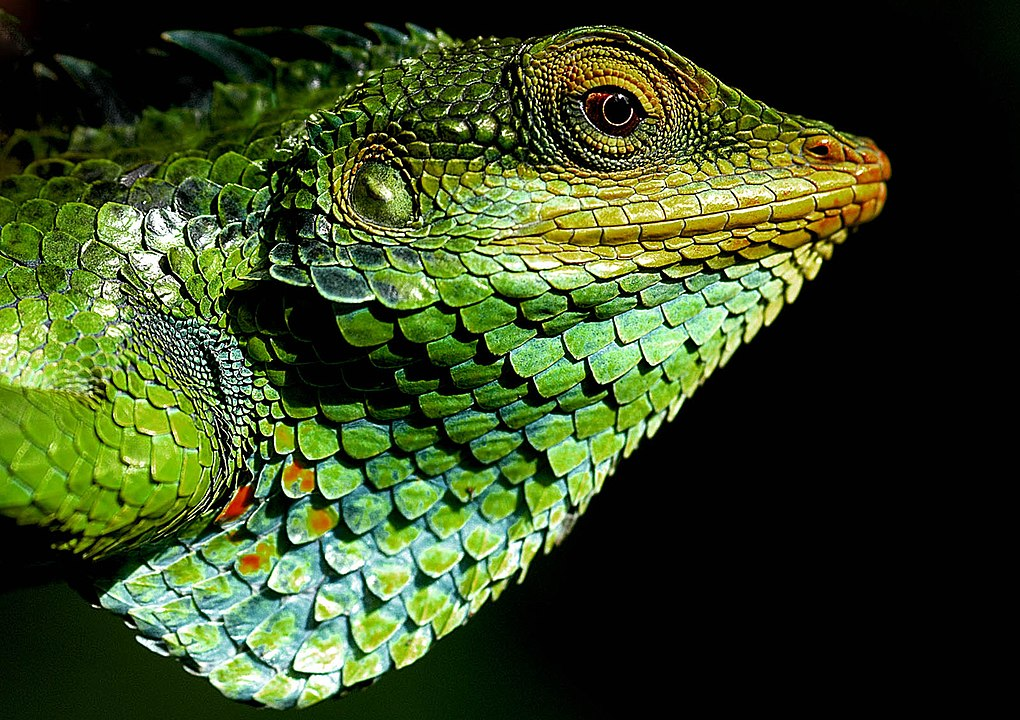
\includegraphics[width=7.5cm]{images/cannyTestImage.jpg}}}
        \caption*{
            \centering Sourced from Wikipedia\textsuperscript{\tiny\textcopyright} \\ \url{https://en.wikipedia.org/wiki/Canny_edge_detector##Walkthrough_of_the_algorithm}
        }
    \end{figure}

    \bk   

    \begin{longtable}{| C{0.6cm} | C{2.5cm} | C{4.75cm} | C{4.75cm} | L{1cm} | L{1.4cm} |}
    \hline
    \multicolumn{6}{| l |}{\textbf{2.4} The edge detection must have the option to be single threaded} \\
    \hline
    \multicolumn{6}{| l |}{\textbf{2.2.1 - 2.2.7} Stages of edge detection.} \\
    \hline
    \rn  & Black and White Method & Canny Edge Detection method should be ran with the original testing image. & \mbox{}{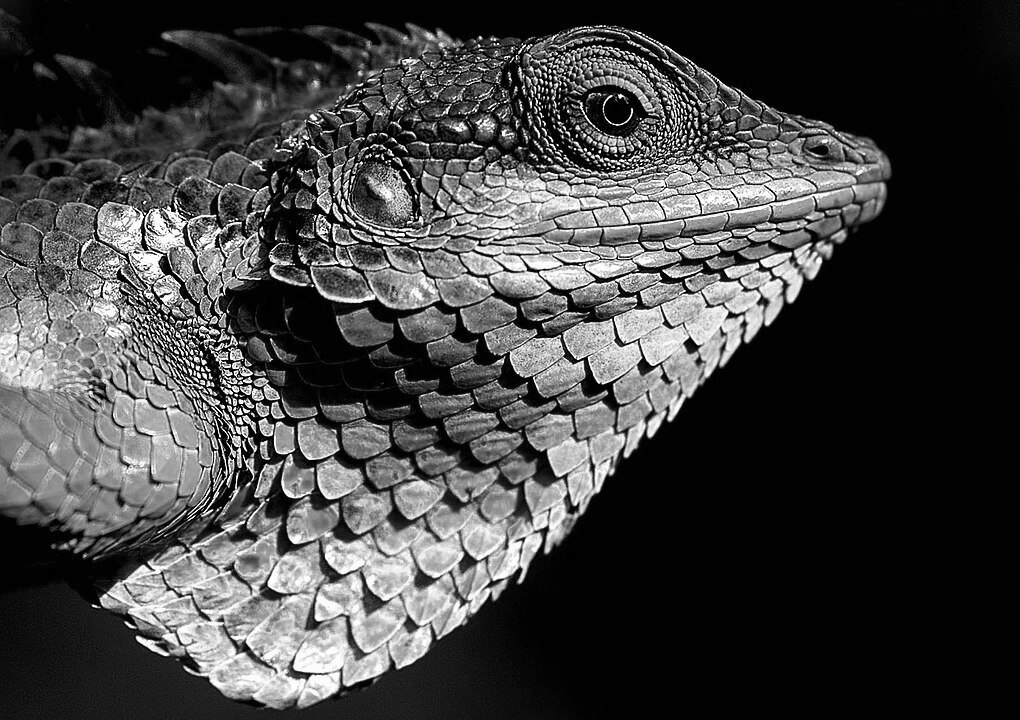
\includegraphics[width=4.5cm]{images/cannyTesting/Canny_Walkthrough_0_Black_White_Filter.jpg }} & Pass & TODO \\
    \hline
    \rn  & Gaussian Filter Method & Canny Edge Detection method should be run with the output of the previous step, Black and White conversion. & \mbox{}{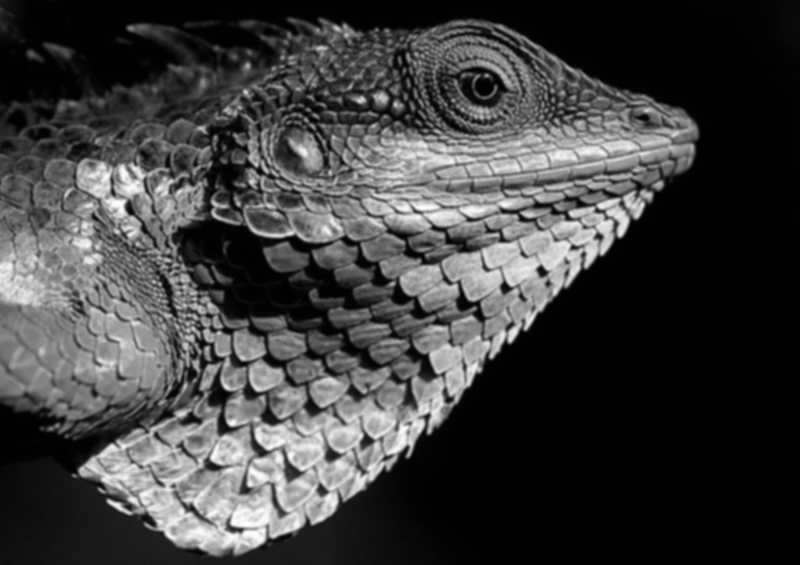
\includegraphics[width=4.5cm]{images/cannyTesting/Canny_Walkthrough_1_Gaussian_Blur.png }} & Pass & TODO \\
    \hline
    \rn  & Gradient Calculation Method(s) & This test describes a series of method calls which will all combine to form the image to the right. During this test, the outputs of each individual method call should be shown. The input into the initial methods should be the output from the Gaussian filter.  & \mbox{}{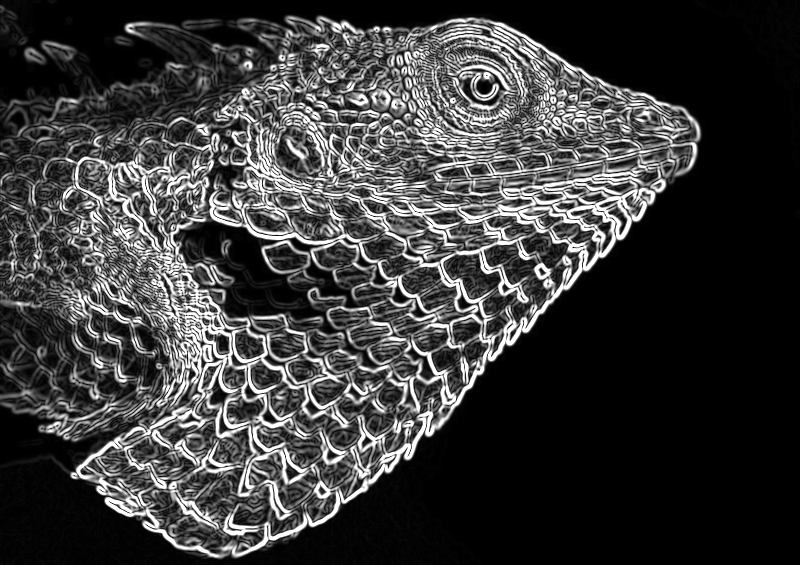
\includegraphics[width=4.5cm]{images/cannyTesting/Canny_Walkthrough_2_Intensity_Gradient.png }} & Pass & TODO \\
    \hline
    \rn  & Gradient Calculation Method & This test describes a series of method calls, the initial calls should be run with the output from the Gaussian filter. & The program should not start the gradient calculations, it should not run any further and should throw an ArgumentException. & Pass & TODO \\
    \hline
    \rn  & Threshold Method(s) & Canny Edge Detection method should be run with the output of the previous successful step, the non-error gradient calculations. & \mbox{}{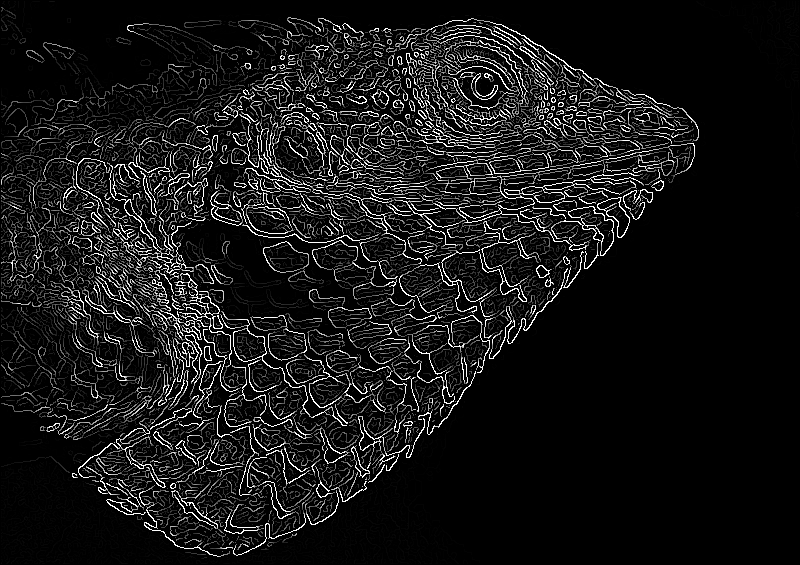
\includegraphics[width=4.5cm]{images/cannyTesting/Canny_Walkthrough_3_Non-maximum_suppression.png }} & Pass & TODO \\
    \hline
    \rn  & Hysteresis Method & Canny Edge Detection method should be run with the output of the previous step, the gradient calculation methods. After this test the image will be in its final edge detected form. & \mbox{}{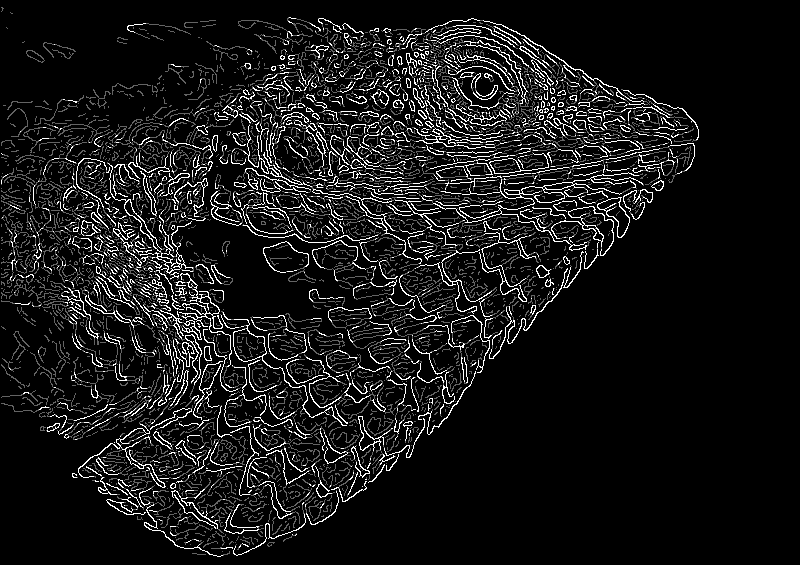
\includegraphics[width=4.5cm]{images/cannyTesting/Canny_Walkthrough_4_Double_Threshold.png }} & Pass & TODO \\
    \hline
    \rn  & Run Full Custom Run (Quick) & Using the "RunQuadrant" method in order to quickly process an image. The default values should be used and the result file should be compared to the image to the right. & \mbox{}{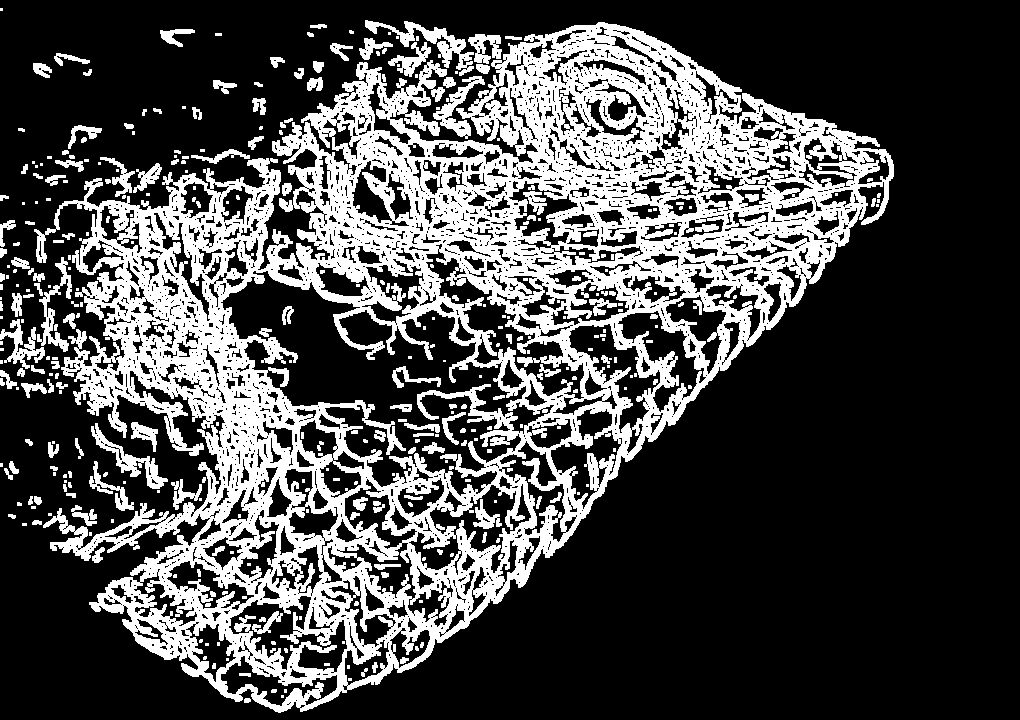
\includegraphics[width=4.5cm]{images/cannyTesting/Canny_Walkthrough_5_Hysteresis.png }} & Pass & TODO \\
    \hline
    \rn  & Run Full Custom Run (Slow) & The slow single threaded version should be used, this should allow the user to change and go back on variables if they do not like the output. The final expected result is seen to the left. At each stage however the processed images should be shown. & \mbox{}{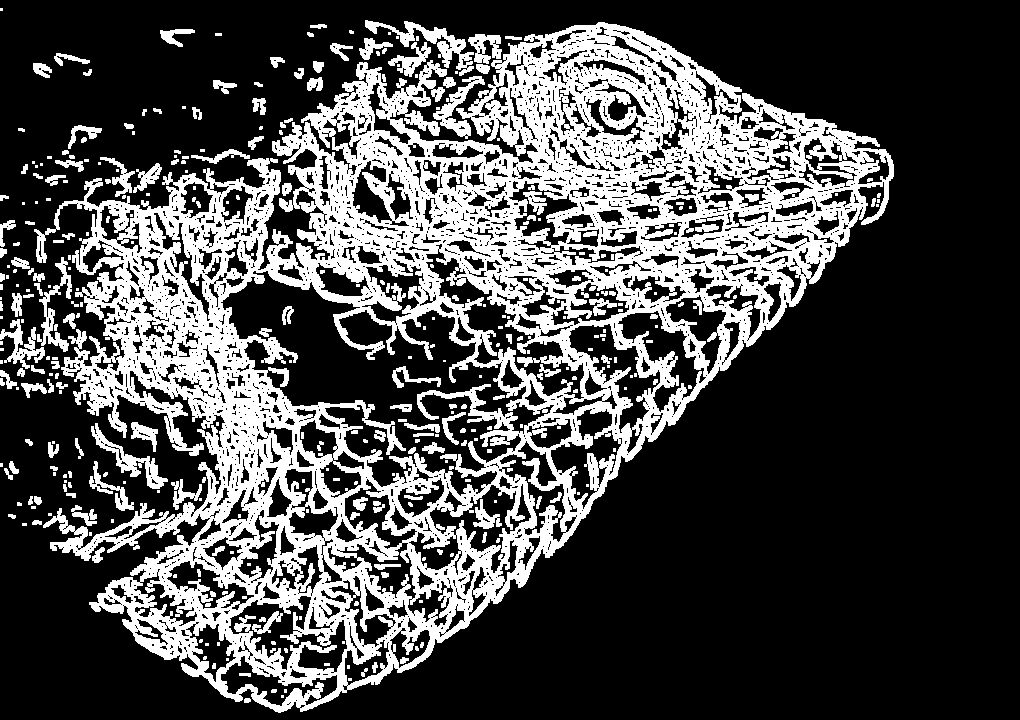
\includegraphics[width=4.5cm]{images/cannyTesting/Canny_Walkthrough_5_Hysteresis.png }} & Pass & TODO \\
    \hline
    \end{longtable}
    \BK





    \setcounter{magicrownumbers}{0}
    \subsubsection{Road Detection and Graph Conversion Testing Table}
    \bk
    \normalsize
    \begin{longtable}{| C{0.6cm} | C{2.5cm} | C{4.75cm} | C{4.75cm} | L{1cm} | L{1.4cm} |}
    \hline
    {\footnotesize Test No.}  & Name & Input Data / Description & Expected Output & Pass Fail & Test Evidence \\
    \hline\hline
    \multicolumn{6}{| l |}{\textbf{3} The Program must overlay the detected roads onto the original imaged} \\
    \multicolumn{6}{| l |}{\textbf{3.2.4 - 3.2.5} The total filled image can be displayed to the user} \\
    \hline
    \rn  & Full Run of Road Detection & Using the test image, after the run of canny edge detection the result should not be inverted and the road threshold should be set to 0.3 and then the road detection run. & \mbox{}{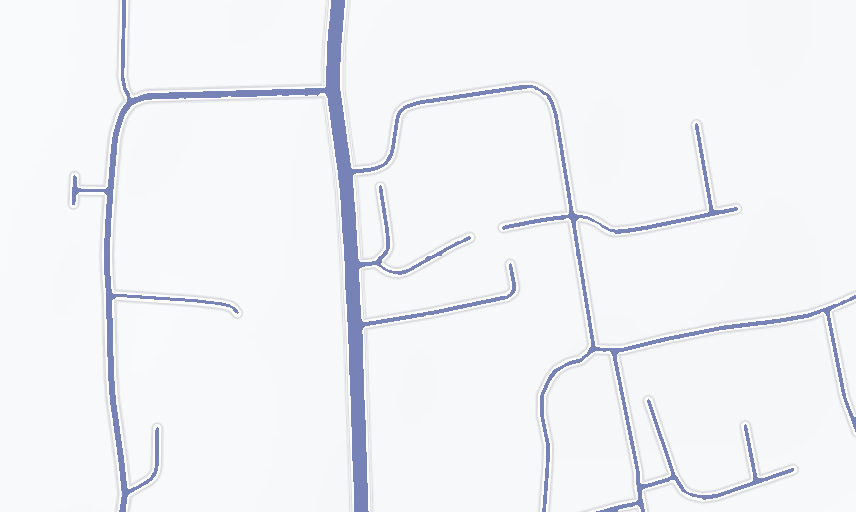
\includegraphics[width=4.5cm]{images/roadExamples/comb.png }} & Pass & TODO \\
    \hline
    \multicolumn{6}{| l |}{\textbf{3.2.3} The percentage threshold for non roads much be changeable by the user } \\
    \hline
    \rn  & Enter Valid Threshold & When the road prompt is shown a number within the shown range should be entered. & The program should accept this new input and use it in the following process. It should also clearly show the user that the value has been changed. & Pass & TODO \\
    \hline
    \rn  & Enter Invalid Threshold & When the road prompt is shown a number out the shown range should be entered as well as this invalid strings should be entered. Examples include "test", "ds@13=kle3q" etc... & The program should use the default value and not error. It should clearly show the user that the default value has been used. & Pass & TODO \\
    \hline
    \rn  & Redo Threshold & After the road detection has been performed the user is prompted whether the result is as they like, at this prompt "No" should be entered. & The program should exit with an error message "You asked for the processing of your map to stop.". It should then return to the main menu. & Pass & TODO \\
    \hline
    \multicolumn{6}{| l |}{\textbf{3.2.1} The image should have the option to be inverted} \\
    \hline
    \rn  & Invert Image Method & An all black image 100x100 image should be fed into this method and then the output should be a 100x100 white square. & \mbox{}{
\includegraphics[width=4.5cm]{images/roadExamples/white.png }} & Pass & TODO \\
    \hline
    \multicolumn{6}{| l |}{\textbf{3.2.2} A filling algorithm should be applied to the image} \\
    \hline
    \rn  & Fill Image Method & An image with 4 white quadrants should be fed into the function. This image should be 200x200. The colours used are pseudo randomly generated so they may not be identical to the expected output, the 4 quadrants should still be filled however. & \mbox{}{
\includegraphics[width=4.5cm]{images/roadExamples/quadsFilledExample.png }} & Pass & TODO \\
    \hline
    
    \end{longtable}
    \BK

    \setcounter{magicrownumbers}{0}
    \subsubsection{Graph Traversal Testing Table}
    \bk
    \normalsize
    \begin{longtable}{| C{0.6cm} | C{2.5cm} | C{4.75cm} | C{4.75cm} | L{1cm} | L{1.4cm} |}
    \hline
    {\footnotesize Test No.}  & Name & Input Data / Description & Expected Output & Pass Fail & Test Evidence \\
    \hline
    \end{longtable}
    \textit{The following are all performed on the test image unless otherwise stated, some of the tests are conducted separate to the main program but still using the same methods and functions. This is due to the fact that some of these traversal algorithms are never shown to the user.} \\
    \bk
    \begin{longtable}{| C{0.6cm} | C{2.5cm} | C{4.75cm} | C{4.75cm} | L{1cm} | L{1.4cm} |}
    \hline
    \multicolumn{6}{| l |}{\textbf{4.1.2}  The Program should Implement Searching Algorithms these do not have to be shown to the user.} \\
    \hline
    \multicolumn{6}{| l |}{\textbf{4.1.2.2}  This includes DFS (Depth-first search).} \\
    \hline
    \rn  & Run DFS & Using the test image run depth first search. Since this test is not shown the user use the premed video. & To the human eye it should look like the path is going "down" more than it is going across, in essence it should look like the image is "filling up". & Pass & TODO \\
    \hline
    \multicolumn{6}{| l |}{\textbf{4.1.2.1}  This includes BFS (Breadth-first search).} \\
    \hline
    \rn  & Run BFS Location 1 & Using the test image run breadth first search. Since this test is not shown the user use the premed video. & To the human eye it should look like the path is going "across" more than it is going down, in essence it should look like something is spreading from a single point source out to the rest of the image. & Pass & TODO \\
    \hline
    \rn  & Run BFS Location 2 & Using the test image run breadth first search. Since this test is not shown the user use the premed video. & To the human eye it should look like the path is going "across" more than it is going down, in essence it should look like something is spreading from a single point source out to the rest of the image. & Pass & TODO \\
    \hline
    \multicolumn{6}{| l |}{\textbf{4.1.1}  The Program should implement Routing Algorithms} \\
    \hline
    \multicolumn{6}{| l |}{\textbf{4.1.1.1}  This includes Dijkstra’s algorithm.}
    \\
    \hline
    \rn  & Run Dijkstra & Using the save.vmap perform graph traversal using the algorithm "Dijkstra's" setting the start node and end node anywhere on the graph then clicking "Pathfind" & The program should perform Dijkstra's algorithm on the image before drawing the path which it found as the most optimal route. & Pass & TODO \\
    \hline
    \rn  & Run Dijkstra Same Start Different End & Using the same start node as the previous test the end node should be moved, then "pathfind" should be clicked & The program should instantly draw the new path without having to re-perform Dijkstra's & Pass & TODO \\
    \hline
    \rn  & Run Dijkstra Different Start Same End & With the same end node as above, the start node should be moved to another point on the image then the "Pathfind" button should be clicked. & The program should perform Dijkstra's again due to the start node being moved. & Pass & TODO \\
    \hline
    \rn  & Run Dijkstra Different Start Different End & Move both the start and end nodes from the ones above and then click "Pathfind" & As above the program will have to recalculate the entire path since the start node has moved. & Pass & TODO \\
    \hline
    \rn  & Run Dijkstra End on Find & Enable the setting "endOnFind" and then perform Dijkstra's on two nodes which are relatively spatially close to each other. Then click "Pathfind". & The program will perform Dijkstra's however if it locates the end node it will pause pathfinding there and stop. It should be faster than regular Dijkstra's & Pass & TODO \\
    \hline
    \multicolumn{6}{| l |}{\textbf{4.1.1.2}  This includes A* (a specialised Dijkstra)}
    \\
    \hline
    \rn  & Run A* Image & Two nodees should be placed on points on the graph, then the "Pathfind" button should be clicked. & The algorithm will run the A* algorithm which using a heuristic algorithm will more efficiently find a path to the end node. It should run faster than Dijkstra's. & Pass & TODO \\
    \hline
    \end{longtable}
    \BK

    \setcounter{magicrownumbers}{0}
    \subsubsection{Logging and Saves Testing Table}
    \bk
    \normalsize
    \begin{longtable}{| C{0.6cm} | C{2.5cm} | C{4.75cm} | C{4.75cm} | L{1cm} | L{1.4cm} |}
    \hline
    {\footnotesize Test No.} & Name & Input Data / Description & Expected Output & Pass Fail & Test Evidence \\
    \hline\hline
    \multicolumn{6}{| l |}{\textbf{8} The program should have re-callable settings} \\
    \hline
    \rn  & Read Normal Settings File & Start the program and navigate to "Settings" & No error should occur and settings should be able to be changed. & Pass & TODO \\
    \hline   
    \rn  & Read Corrupt Settings File & Remove and rename sections of settings file. Then as above. & The program should error and instruct the user how to correct the fault. & Pass & TODO \\ 
    \hline
    \rn  & Programmatically Alter Normal Settings File & Navigate to "Settings" and change settings in each sub menu and show altered settings.conf & settings.conf should show the changed settings. Before and after should be shown side by side. & Pass & TODO \\
    \hline
    \rn  & Programmatically Alter Corrupt Settings File & Remove entry from settings then attempt to alter settings similar to above. & The program should error and instruct the user how to correct the fault. & Pass & TODO \\
    \hline
    \rn  & Save Corrupt Settings File & Attempt to enter the settings menu, alter a setting and the exit. Upon the "exit" condition the file will be saved. & The program should not let the user alter the settings and should error and instruct the user how to proceed. & Pass & TODO \\
    \hline
    \rn  & Save Normal Settings File & Enter the settings menu, alter a setting and then exit. Upon the "exit" condition the file will be saved. & The file should save without issue and a side by side of the programmatically altered file should be shown. & Pass & TODO \\
    \hline
    \rn  & Manually Alter Settings File & Open the settings.conf file and change settings values then save and restart the program. Once the program has been restarted check the settings in the menu to see if they have been changed. & The changed settings state should be mirrored in the settings menu. & Pass & TODO \\
    \hline
    \multicolumn{6}{| l |}{\textbf{9 / 10}  The program settings / save files should be easily movable. } \\
    \hline
    \rn  & Run Program Fresh & Run the executable of the program. & In the file directory 3 folders should be created. Runs, Saves, Logs. And inside of the log file there should be a file called master.txt Inside the master log a startup message should be recorded. There should also be a config file created. & Pass & TODO \\
    \hline
    \rn  & Re-run Program & Close the program which was just started. Then run the executable. & No files should be created or deleted however there should be a new entry in the master.log & Pass & TODO \\
    \hline
    \rn  & Delete Some Folders and Re-run & In the directory where the program file is contained the programatically created folders should be deleted. Not all but some. & When the program is restarted the files should be recreated & Pass & TODO \\
    \hline
    \rn  & Full Run and Check Master Log & After the previous tests have been completed (ones involving a raw image being processed) the master.log should be checked & when checking the master log there should be a message saying that a run has started and that it ends. Furthermore it should contain the ID of the run. & Pass & TODO \\
    \hline
    \rn  & Full Run and Check Individual Log & After the previous tests have been completed (ones involving a raw image being processed) the individual unique run log should be checked & Inside the per run log there should be each step of the edge detection and others depending on pathfinding. & Pass & TODO \\
    \hline
    \rn  & Cause Error and Check Log & Check the log after one of the input validation tests. & There should be a line in the master file referencing the error. & Pass & TODO \\
    \hline
    \multicolumn{6}{| l |}{\textbf{7.1} The map in a binary file format } \\
    \hline
    \multicolumn{6}{| l |}{\textbf{7.2} The saved images from the processing of the map should be able to be saved in a  } \\
    \multicolumn{6}{| l |}{ compressed format. } \\
    \hline
    \rn  & Full Run with Save To Zip & Process a whole image asking for it to be saved. The setting "zipOnComplete" enabled. This will ensure that after the processing the file is saved. & After the run has completed in the root directory a zip file will be created containing any partial images, save file and logs. & Pass & TODO \\
    \hline
    \rn  & Run with Detailed Logging & Enable the setting "detailedLogging" and run through a full process of map recognition. & To the side of the main screen during the process detailed log messages of what exactly is going on should be shown. & Pass & TODO \\
    \hline

    \rn  & View Save File From Program & Using the test image save attempt to read it into the program. & The program should accept the test image save and take the user to the save image file. & Pass & TODO \\
    \hline
    \multicolumn{6}{| l |}{\textbf{7.6} The saved binary file should be able to be have its description changed } \\
    \hline
    \rn  & Change Save File Information & First the file information should be viewed by selecting "View File Information" then once what you know what you wish to change the "Change File Information". Then any of the details may be changed. & Once a change has been made the program should create a copy of the save file with the new info contained within and the rest of the old data. & Pass & TODO \\
    \hline
    \multicolumn{6}{| l |}{\textbf{7.3} The saved binary file should be able to be cloned } \\
    \hline
    \rn  & Clone Save File & On the save file info page select "Clone" & The program should create a copy of the save file with all of its details exactly the same. & Pass & TODO \\
    \hline
    \multicolumn{6}{| l |}{\textbf{7.5} The saved binary file should be able to be renamed } \\
    \hline
    \rn  & Rename Save File & In the save file menu, "Rename" should be selected. A new name should be entered. & The program will be renamed to the value which the user entered. & Pass & TODO \\
    \hline
    \multicolumn{6}{| l |}{\textbf{7.7} The saved binary file should be able to be able to be deleted } \\
\hline
    \rn  & Delete Save File & As above select "Delete" and then follow the prompts to delete the file. & Once the user has navigated to the confirm button the program will delete the save file. & Pass & TODO \\
    \hline
    \rn  & Recall to Pathfind Save File & In the recalled options select the pathfind option. & When this option is selected the program will turn over to the pathfinding image form. From there the user can perform graph traversal on it. & Pass & TODO \\
    \hline
    \end{longtable}
    \BK

    \setcounter{magicrownumbers}{0}
    \subsubsection{Miscellaneous Testing Table}
    \bk
    \normalsize
    \begin{longtable}{| C{0.6cm} | C{2.5cm} | C{4.75cm} | C{4.75cm} | L{1cm} | L{1.4cm} |}
    \hline
    {\footnotesize Test No.}  &  Name & Input Data / Description & Expected Output & Pass Fail & Test Evidence \\
    \hline\hline
    \multicolumn{6}{| l |}{ \normalsize{\textbf{6.1}:The program must implement a matrix class } } \\
    \hline
    \rn  & Matrix Constructor & b & c & Pass & TODO \\
    \hline
    \rn  & Array Index Accessing of Matrix & b & c & Pass & TODO \\
    \hline
    \rn  & Adding Matrices & b & c & Pass & TODO \\
    \hline
    \rn  & Subtracting Matrices & b & c & Pass & TODO \\
    \hline
    \rn  & Matrix Multiplication & b & c & Pass & TODO \\
    \hline
    \rn  & Scalar Multiplication & b & c & Pass & TODO \\
    \hline
    \rn  & Matrix Minimisation & b & c & Pass & TODO \\
    \hline
    \rn  & Matrix Convolution & b & c & Pass & TODO \\
    \hline
    \multicolumn{6}{| l |}{ \normalsize{\textbf{X.X}: No set objective but contribute to the simplistic and user input objectives} } \\
    \hline
    \rn  & Progress Bar Creation & b & c & Pass & TODO \\
    \hline
    \rn  & Progress Bar Update Action & b & c & Pass & TODO \\
    \hline
    \rn  & Coord Struct ToString & b & c & Pass & TODO \\
    \hline
    \rn  & Coord Struct Equals Method & b & c & Pass & TODO \\
    \hline
    \rn  & Coord Struct Equals Opperator & b & c & Pass & TODO \\
    \hline
    \rn  & Coord Struct Not Equals Opperator & b & c & Pass & TODO \\
    \hline
    \rn  & 2D Double Array ToBitmap Extension & b & c & Pass & TODO \\
    \hline
    \rn  & Bitmap ToDoubles Extension & b & c & Pass & TODO \\
    \hline
    \rn  & 2D RGB Structure ToBitmap Extension & b & c & Pass & TODO \\
    \hline
    \rn  & 2D Doubles ToGraph & b & c & Pass & TODO \\
    \hline
    \rn  & SetPixel Extension & b & c & Pass & TODO \\
    \hline
    \rn  & GetPixel Extension & b & c & Pass & TODO \\
    \hline
    \rn  & Gaussian Distribution Utility & b & c & Pass & TODO \\
    \hline
    \rn  & Bound Utility & b & c & Pass & TODO \\
    \hline
    \rn  & TryBound Utility & b & c & Pass & TODO \\
    \hline
    \rn  & Degree to Radian Utility & b & c & Pass & TODO \\
    \hline
    \rn  & Radian to Degree Utility & b & c & Pass & TODO \\
    \hline
    \rn  & Map Radian To Pixel Utility & b & c & Pass & TODO \\
    \hline
    \rn  & Combine Bitmap Utility & b & c & Pass & TODO \\
    \hline
    \rn  & Split Image Utility & b & c & Pass & TODO \\
    \hline
    \rn  & combine Quadrants Utility & b & c & Pass & TODO \\
    \hline
    \rn  & Inverse Image Utility & b & c & Pass & TODO \\
    \hline
    \rn  & Generic Rebuild Path Utility & b & c & Pass & TODO \\
    \hline
    \rn  & Is Yes Utility & b & c & Pass & TODO \\
    \hline 
    \rn  & Get Red Utility & b & c & Pass & TODO \\
    \hline
    \rn  & Get Green Utility & b & c & Pass & TODO \\
    \hline
    \rn  & Get Blue Utility & b & c & Pass & TODO \\
    \hline
    \rn  & Get Average Utility & b & c & Pass & TODO \\
    \hline
    \rn  & Get Industry Average Utility & b & c & Pass & TODO \\
    \hline
    \rn  & Get If Exists Utility & b & c & Pass & TODO \\
    \hline
    \rn  & Get Distance Between Nodes Utility & b & c & Pass & TODO \\
    \hline
    \end{longtable}
    \textit{The following tests refer to pathfinding through any given map using A-Star, this is testing the "Pathfind Image Form". The test image recalled from a save file will be used for all of these tests unless otherwise specified.} \\ \bk
    \begin{longtable}{| C{0.6cm} | C{2.5cm} | C{4.75cm} | C{4.75cm} | L{1cm} | L{1.4cm} |}
    \hline
    \multicolumn{6}{| l |}{\textbf{5} | The Program must have a Clear and Simplistic GUI.} \\
    \multicolumn{6}{| l |} {\textbf{5} | (The following show that it is easy to use and hard to break the user inputs.)} \\
    \hline
    \rn  & Select No Nodes & Neither left or right mouse buttons should be clicked and then the "Pathfind" button should be clicked. & The program should not run and instantly go back to waiting for input. & Pass & TODO \\
    \hline
    \rn  & Select One Node & Only one left or right mouse button should be clicked and then the "Pathfind" button should be clicked. & The program should not run and instantly go back to waiting for input. & Pass & TODO \\ 
    \hline
    \rn  & Select Two Nodes & Neither left or right mouse buttons should be clicked and then the "Pathfind" button should be clicked. & The program should run and after some time should then wait for input. & Pass & TODO \\
    \hline
    \rn  & Select One Node Off Path & First the "snapToGrid" setting to false. Set one node off the path and one on and then click the "Pathfind" button. & The program should not run and instantly go back to waiting for input. & Pass & TODO \\
    \hline
    \rn  & Select Two Nodes Off Path & First the "snapToGrid" setting to false. Set both nodes off the path and then click the "Pathfind" button. & The program should not run and instantly go back to waiting for input. & Pass & TODO \\
    \hline
    \rn  & Select One Node Off Path One On with Dijkstras & First the "snapToGrid" setting to false. Set one node off the path and one on and then click the "Pathfind" button. & The program should run momentarily and allow then return to waiting. If the end node is then placed back on the road the pathfinding should be instant. & Pass & TODO \\
    \hline
    \rn  & Click Continue Button in View Image Form & Get to a situation where the "View Image" form is shown. This can be during Canny Edge Detection or when a new image is processed. Then click the continue button. & The button should cause the form to close itself and allow the program to continue. & Pass & TODO \\
    \hline
    \end{longtable}
    \BK

    \subsection{Testing Video}
        Please find below several links to the NEA testing video as well as a QR code. The timestamps from the table refer to points in this video. Timestamps are also contained within the description. \\ \bk
        
        \begin{center}
            \quad
            \qrcode{https://youtu.be/cJqFovg27Bo}
            \\ \BK
            \large
            \text{Raw URL: \url{https://youtu.be/cJqFovg27Bo}} \\            
            \normalsizeer
            \textit{charlie JULIET quebec FOXTROT oscar victor golf two seven BRAVO oscar} \\ \bk  
            \large
            \text{Short URL: \url{https://shorturl.at/dT158}} \\
            \normalsizeer
            \textit{delta TANGO one five eight}
        \end{center}        
\end{flushleft}